\documentclass[12pt,a4paper]{article}

\usepackage{amsmath}
\usepackage{amsfonts}
%\usepackage{mitpress}
\usepackage{amssymb}
\usepackage[USenglish]{babel}
%\usepackage{enumerate}
\usepackage{graphicx}
\usepackage{booktabs}
\usepackage[utf8]{inputenc}
\usepackage{siunitx}
\usepackage{natbib}
\bibliographystyle{agsm}
%\usepackage{caption} 
%\captionsetup[table]{skip=10pt}
\usepackage{threeparttable}
\usepackage{caption}

\newtheorem{theorem}{Theorem}
%\newtheorem{acknowledgement}{Acknowledgement}
\newtheorem{algorithm}{Algorithm}
\newtheorem{assumption}{Assumption}
\newtheorem{axiom}{Axiom}
\newtheorem{case}{Case}
\newtheorem{claim}{Claim}
\newtheorem{conclusion}{Conclusion}
\newtheorem{condition}{Condition}
\newtheorem{conjecture}{Conjecture}
\newtheorem{corollary}{Corollary}
\newtheorem{criterion}{Criterion}
%\theoremstyle{definition}
\newtheorem{definition}{Definition}
\newtheorem{example}{Example}
\newtheorem{exercise}{Exercise}
\newtheorem{lemma}{Lemma}
\newtheorem{notation}{Notation}
\newtheorem{problem}{Problem}
\newtheorem{proposition}{Proposition}
\newtheorem{remark}{Remark}
\newtheorem{solution}{Solution}
\newtheorem{summary}{Summary}
\newtheorem{fact}{Fact}

\begin{document}

%Foreign Firms, Expatriate Managers: Accounting for the Effects of Domestic and Foreign CEOs in Hungarian Enterprsies
\title{Good Owners, Choose Successful Managers: Accounting for the Effects of Local and Expatriate Managers in Foreign Enterprises\thanks{This research was funded by the European Research Council (ERC Starting Grant agreement number 313164). The managerial database used in this paper was developed by the team of the CEU Mircodata Laboratory (Krisztián Fekete, Olivér Kiss, Bálint Szilágyi, András Vereckei and Rita Zágoni). We thank the excellent research assistance of Szilárd Perédi and Gergő Závecz. The paper benefited from presentations at the Lunch Seminar of the CEU Department of Economics and the London School of Economics. The views expressed in this paper are those of the authors and do not necessary reflect the official view of the European Research Council or the National Bank of Hungary. All errors are our own.}

\newline\\\small{PRELIMINARY VERSION}}

\author{Miklós Koren\thanks{Koren: Central European University, Intitute of Economics -- HAS and CEPR. 1051 Budapest, Nádor u. 9., Hungary. E-mail: korenm@ceu.edu.} \and Álmos Telegdy\thanks{Telegdy: National Bank of Hungary, Central European University and Institute of Economics -- HAS. 1054 Budapest, Szabadság tér 9. E-mail: telegdya@mnb.hu}}

\date{March 2019}
\maketitle

\begin{abstract}
Using exhaustive administrative data from Hungary on the universe of firms over 20 employees and their managers for 1980-2015, we study how Chief Executive Officers (CEOs) elected by foreign owners affect the performance of firms. Using 1,796 foreign acquisitions out of which about 1,400 replace their CEO after the foreign takeover of whom 750 are expatriates and the others local managers, we employ difference-in-differences techniques to compare foreign firms that do not change their CEO, replace their CEO with a domestic individual, and replace the CEO with an expatriate. We find that CEOs employed after the foreign acquisition increase the scale of production and labor productivity by 6.5 percent. Expatriate CEOs have an additional scale effect of 10 percent and productivity effect of 6.5 percent. The reasons for this increase are not inputs as neither labor nor capital changes, but newly hired CEOs engage actively in exporting which increases by 9 percent for foreign-hired CEOs and by an additional 13 percent for expatriates.
\end{abstract}

Firms differ vastly in productivity even within narrowly defined industries (\cite{Syverson2011-ti}), and one reason for this difference is the identity of the firm's owner. A large literature documents that subsidiaries of multinationals and other foreign-owned firms are more productive than local firms (see \cite{Doms1998-su,Barba_Navaretti2004-cs}. This observed difference may partly be the result of selection as firms that expand across national borders are better than those which do not, but the literature suggests that the productivity gap is at least partly causal \cite{Arnold2009-so}.\footnote{In the CEE context, \cite{Javorcik2004-gz} studies productivity spillovers in Lithuania, while \cite{David_Brown2010-iz,Brown2006-rn} study the effects of foreign privatization acquisitions on productivity, employment and wages in four transition countries. Regarding parent effects, \cite{Javorcik2011-uj} show that American and European foreign companies behave differently in Romania, consistently with tariff incentives.} 

Several mechanisms may account for the superior performance of foreign-owned enterprises. Multinational companies have access to the newest technologies that let them reach the frontier of production possibilities \cite{guadalupe2012innovation}. Financially healthy parent companies can provide their subsidiaries with fresh capital, a prerequisite for growth\cite{levine2005finance}. Foreign companies may also be more able to staff their subsidiaries with good managers. Good general ability of managers, or some specific knowledge of managers that is valuable to the firm (like the know-how of exporting) can foster growth and improve firm performance \cite{Bertrand2003-io, Bloom2010-je,Bloom2012-ek,Bloom2014-ux}.\footnote{The large increase in the level and inequality of CEO pay \cite{frydman2010executive} also suggests that the returns to good management are large.}

In this paper we go beyond the traditional analysis of foreign ownership when the firm is seen as a black box and ownership is proxied by either a dummy variable or the ownership share of foreign owners, and explore the effect of the expatriate chief executive officers (CEOs) on firm outcomes.\footnote{The period covered by our data, especially the nineties, involved rapid liberalization of the business environment. The new business opportunities combined with the government's bolstering of foreign direct investment (FDI) brought about a very large number of firms acquired by foreigners and green-field investments alike. This institutional arrangement places Hungary among the most suitable countries to study of the effects of FDI.} For this purpose we build a novel dataset of managers of all firms incorporated in Hungary for the period 1992--2016. To study firm performance, we link this dataset to balance sheet information of the population of Hungarian firms for the years between 1980 and 2015.\footnote{Throughout the analysis we drop firms under 20 employees as expat management is relatively scarce among them and the quality of data in the microfirms is lower than in larger businesses.}

We identify managers from administrative data which includes the names and home addresses of firm representatives. We classify a manager as foreign if she has a foreign address or has a non-Hungarian name.\footnote{Because Hungarians use the Eastern name order (surname first, given name last) and given names are officially regulated as they can be chosen from closed list, Hungarian names can be identified with great accuracy. For example, ``Bauer Éva'' will be classified Hungarian, whereas ``Eva Bauer'' foreign.} By the end of our sample, around 15 percent of firms had exposure to foreign managers and these these firms are predominantly foreign-owned.

To differentiate the causes and effects of foreign ownership from those of foreign management, we focus on three groups of firms defined by their main owner, each operating with an expatriate or local CEO. The first group includes firms that have been acquired by a foreign investor; the second is the set of greenfield investments initiated by foreign owners; and the third group is made of the domestically owned firms.

%talk on selection: only foreign firms have expats, median size small, positive selection
We first study which firms have a foreign CEO. Foreign owned firms may place an expatriate as a CEO for several reasons.  Expatriates may possess more general skills (because having better education or more expertize) and thus be more able to run the subsidiary. If the subsidiary needs some special skill (for example, it wants to enter the international markets) and foreign CEO may have more expertize in this activity and thus is more suited to run the company.  In addition to ability, a person who served for the parent company (as a manager, for example), is more knowledgeable of the internal processes of the firm which is an advantage compared to a local manager.  Finally, the company's owners may trust more a manager who was with the firm already. The downside of expatriates is that they tend to be very expensive both in salaries and fixed costs of transfer from the home to the source country.  In addition, many foreign managers burn out prematurely under the stressful conditions of the foreign environment which puts a burden on the company by losing the sunk costs of expatriation.

To analyze which foreign-owned firms have a foreign CEO, we use simple cross-section regressions on the sample of to-be-acquired firms to predict the arrival of a foreign manager within the next two years. Greenfield FDIs are the most likely to have an expatriate manager, followed by foreign acquisitions.  Larger firms (as measured by employment and output) are less likely to get an expatriate CEO.  Those with high capital stock and which export are more prone to having one.  There are also notable differences across investor source countries.

We next study firm outcomes with and without expatriate managers. Here we use a differences-in-differences strategy and compare foreign to domestically managed firms before and after the arrival of new management. We test the effect of expatriate managers on a wide variety of firm outcomes, including changes in input and output levels (labor, investment and value of sales), changes in technology (proxied by the K--L ratio), productivity (labor productivity and total factor productivity), survival and exporting.  In the sample where we have access to worker data we also look at other measures of restructuring, such as the ratio of high-skilled workers and churning of the workforce.  We find that, expatriate CEOs raise labor and the value of output such that labor productivity also increases.  They, however, do not have an effect on the exporting activity of the company and decrease the capital-labor ratio of the firm (which we use to proxy the technological level of the firm). When investigate the differences of foreign management in domestic, greenfield and acquired firms, we find that in domestic firms it has an effect only on exporting and in acquisitions on all the outcome variable.  Acquired firms under foreign management increase their output and labor productivity more than those which are managed by a Hungarian CEO.\footnote{These findings are robust to different sample definitions, such as the disaggregation of the population of firms into manufacturing and services or slicing the data into early and late periods.} Our findings suggest that investors follow distinct strategies when investing in Hungarian firms. 

Our work uncovers a mechanism which can explain -- albeit partially -- the superior performance of foreign-owned enterprises and we also provide new facts about the role of expatriate managers for firm performance. The  findings can help evaluate the relative efficacy of trade, FDI, and immigration policies of high-skilled individuals in promoting economic growth. For example, if expatriate managers contribute largely to knowledge flows, then immigration restrictions are harmful to growth (see \cite{Kerr2010-le} on the effects of visa restrictions on scientists and engineers). 

\section{Data and Descriptive Statistics}
For the analysis of expatriate CEO effects we developed a novel dataset which provides information on all managers of Hungarian companies for the period of 1992-2016. Each company has to register all the individuals with signatory rights at the Company Court. These information are stored in a sequence of strings and provides the name and of the individual, her mother's maiden name, the position occupied in the firm, the starting and closing the date of the data entry (see Table \ref{table:rawdata}).\footnote{Although the data start in 1992, the starting dates of the managers with a company are recorded even if they happened before 1992, if the manager was with the company in 1992.}
%Describe data construction process.

\begin{table}[h!]
\caption{Shape of the Raw Data}
\label{table:rawdata}
\centering
\texttt{firm,manager,from,to\\
123456,Gyöngyi,1992-01-01,1996-12-31\\
123456,Georg,1997-01-01,1999-12-31}
\begin{tablenotes}
			\small
      \item {Notes: the table presents two entries that identify managerial names and tenures in a given firm as they are in the Company Court Enterprise Database}.
    \end{tablenotes}
\end{table}

The Hungarian regulation constrains the use of given names for its citizens, as names can be chosen from a closed list.\footnote{(If parents belong to an ethnic minority, they may choose any name for their offspring. Since Hungary is fairly homogenous ethnically and most parents choose typical names, this is not a serious problem in the data.}  In addition, Hungarians use the Eastern name order (surname first, given name last).\footnote{For example, Bauer Éva would be inferred as Hungarian while Eva Bauer as an expatriate.} The data also has  information on the address of the individual. We use these three pieces of information to identify Hungarians. Those who are not identified as Hungarians can be of three distinct categories: firm liquidators and foreign managers.  As liquidators are legal entities, we can distinguish them by searching for indicators for businesses such as \emph{ltd}, \emph{jcs}, etc. Those entries, which are left in the data after removing Hungarians and firms, are coded as foreign.

Firm representatives can be officers of the company (including the CEO) and also employees with signatory rights.  We classify a representative as CEO if either the data entry has this information or she is the sole manager in that year. We create a panel from these data by recording for each manager the company she worked for and her position on June 21st of each year.\footnote{As the balance sheet data have a yearly frequency, there is no reason to use within-firm changes of the management.} The resulting data have information on %add descs.

We link the managerial data to the Hungarian Balance Sheet Database (gathered by the Tax and Customs Office), which contain the financial statements of each Hungarian double-entry book keeping firm for the period between 1980 and 2014, as well as several other variables (such as the location and main activity of the firm, its ownership structure and level of employment).  We have data on 819,000 firms for a total of 6.9 million firm-years. From the universe we keep only those firms which had an average employment of 20 or more in our sample period, did not belong to the financial sector, had at most 15 CEOs during the studied period and we only use firm-years with non-missing data for employment, sales, the value of tangible assets export sales.\footnote{XX is not available before 1992.} To simplify the analysis, we drop always domestic firms with expatriate CEOs as the number of such firms is minuscule (only XX). The final sample has more than 25,000 firms that are observed for 11 years on average and they are linked to XX managers.

%add descriptives

\begin{table}[h!]
\begin{threeparttable}
\centering
\caption{Numbers of Observations by Ownership and Management Type}
\label{table:nobs}
\begin{tabular}{1111111} 
\hline
~     & \multicolumn{2}{l}{Acquisition} & \multicolumn{2}{l}{Greenfield} & \multicolumn{2}{l}{Domestic}  \\ 
\hline
~     & Expat & Local                   & Expat & Local                  & Expat & Local                 \\ 
\hline
1992  & 30    & 690                     & 329   & 689                    & 69    & 7509                  \\
1993  & 74    & 796                     & 465   & 823                    & 91    & 8411                  \\
1994  & 104   & 891                     & 623   & 907                    & 108   & 8741                  \\
1995  & 136   & 941                     & 758   & 932                    & 114   & 8782                  \\
1996  & 160   & 949                     & 839   & 946                    & 120   & 8932                  \\
1997  & 183   & 994                     & 943   & 1016                   & 138   & 9161                  \\
1998  & 226   & 1008                    & 1125  & 988                    & 148   & 9572                  \\
1999  & 291   & 950                     & 1293  & 892                    & 175   & 9603                  \\
2000  & 307   & 926                     & 1484  & 813                    & 195   & 9674                  \\
2001  & 327   & 918                     & 1564  & 781                    & 216   & 9730                  \\
2002  & 329   & 906                     & 1624  & 752                    & 235   & 9772                  \\
2003  & 339   & 884                     & 1639  & 720                    & 248   & 9715                  \\
2004  & 357   & 857                     & 1707  & 692                    & 270   & 9683                  \\
2005  & 379   & 835                     & 1755  & 669                    & 274   & 9542                  \\
2006  & 384   & 798                     & 1822  & 646                    & 286   & 9465                  \\
2007  & 369   & 764                     & 1859  & 622                    & 310   & 9287                  \\
2008  & 388   & 726                     & 1883  & 623                    & 330   & 9095                  \\
2009  & 390   & 685                     & 1877  & 611                    & 321   & 8790                  \\
2010  & 387   & 643                     & 1892  & 606                    & 350   & 8641                  \\
2011  & 392   & 613                     & 1884  & 602                    & 353   & 8456                  \\
2012  & 384   & 584                     & 1891  & 578                    & 348   & 8194                  \\
2013  & 350   & 533                     & 1639  & 538                    & 332   & 7940                  \\
2014  & 340   & 516                     & 1562  & 521                    & 320   & 7618                  \\ 
\hline
\end{tabular}
\begin{tablenotes}
			\small
      \item Notes: the table presents the number of firms by ownership and management. A firm is foreign-owned if its direct of ultimate majority owners are of foreign origin. Acquisition = the firm was domestic and became foreign-owned; Greenfield = the firm entered the data as foreign-owned. Domestic = the firm was owned by Hungarian owners. Expatriate = the CEO of the firm is foreign; Local = the CEO of the firm is Hungarian}.
    \end{tablenotes}
\end{threeparttable}
\end{table}

The resulting sample is summarized in Table \ref{table:nobs}. As expected, most firms are domestically owned and led by a Hungarian CEO, but the fraction of foreign-owned firms is also large and has a positive trend, increasing their presence from about 10 to 20 percent.\footnote{We ignore divestments for now.} The fraction of firms with an expatriate CEO has increased from 4 percent to 15 percent. The largest fraction of expatriate CEOs are in foreign greenfield firms but they are also quite numerous in foreign acquisitions.  Most domestic firms are managed by a Hungarian CEO, but a minority of them employed expatriates.\footnote{Our estimation method identifies the effect of expatriate CEO from firms changing their manager. The number of such firms equals 1,625, with 519 in acquired firms, 740 in greenfield FDIs and 366 in domestically owned enterprises.}

We define several dependent variables.  Employment is the average employment size of the firm, output is the value of sales deflated by implicit industry-level price deflators, assets are the value of tangible assets, exporter is a dummy variable that equals 1 if the firm exports in the given year and investment is a computed variable from assets that has three values.  It equals 1 if the firm increased the value of tangible assets by more than 10 percent from one year to the next, -1 if it decreased it by at least 10 percent, and 0 if its change was less than 10 percent. The descriptive statistics of these dependent variables are presented in Table \ref{table:desc} by firm type (acquisition, greenfield and domestic) and by the provenience of the CEO (expatriate or local).  The table presents the means and standard deviations for these variables by firm-type.  For example, if a firm was acquired by a foreign owner and was managed by an expatriate, all its years (including those before the acquisition) are presented in the first line of the table. The results show that firms that were managed by expatriates during the period of observation tend to be larger by both inputs and the value of sales, are more likely to export but have very similar mean investment than those which were always managed by a Hungarian CEO.

\begin{table}
\caption{Descriptive Statistics by Ownership and Management}
\label{table:desc}
\centering
\begin{tabular}{lllllll} 
\hline
~           & Emp.     & Output     & Assets     & Exporter & Inv.  \\ 
\hline
Acquisition & ~        & ~          & ~          & ~        & ~     \\ 
\hline
Expatriate  & 235.59   & 8916       & 2571       & .65      & .16   \\
~           & (885.72) & (8.11e+04) & (1.67e+04) & ~        & ~     \\
Local       & 194.87   & 4652       & 2162       & .53      & .13   \\
~           & (607.23) & (2.18e+04) & (1.68e+04) & ~        & ~     \\ 
\hline
Greenfield  & ~        & ~          & ~          & ~        & ~     \\ 
\hline
Expatriate  & 172.35   & 7431       & 1767       & .79      & .14   \\
~           & (561.72) & (4.40e+04) & (1.22e+04) & ~        & ~     \\
Local       & 125.53   & 4140       & 1283       & .66      & .14   \\
~           & (271.51) & (1.92e+04) & (1.15e+04) & ~        & ~     \\ 
\hline
Domestic    & ~        & ~          & ~          & ~        & ~     \\ 
\hline
Expatriate  & 156.55   & 3219       & 2048       & .38      & .15   \\
~           & (387.82) & (1.43e+04) & (1.50e+04) & ~        & ~     \\
Local       & 91.30    & 863        & 401        & .31      & .15   \\
~           & (730.44) & (5345)     & (7695)     & ~        & ~     \\ 
\hline
Total       & 115.63   & 2402       & 832        & .41      & .15   \\
~           & (689.93) & (2.35e+04) & (9934)     & ~        & ~     \\
\hline
\end{tabular}
\begin{tablenotes}
			\small
      \item Notes: N = 286,121. The table presents descriptive statistics of firm characteristics.}
    \end{tablenotes}
\end{table}

We define foreign ownership on the basis of majority foreign ownership.\footnote{As most foreign-owned firms are 100 percent owned by foreign investors, alternative cutoffs used in the literature (such as 10 percent), alters foreign categorization to a small extent.} For about half of the firms, the data provide the addresses of owners so we can identify the country of origin of the investors.
%add descriptives of managers

\section{Methodology}
Our goal is to study the performance enhancement of foreign ownership through the management channel. For this purpose first we show that foreign acquisitions indeed increase firm performance in our data as well as in many other analyses (ref). The following difference-in-differences regression equation identifies the foreign ownership effect:
\begin{equation}
	Y_{jkt} = \gamma_F F_{jkt} + f(age_{jt}) + ind_{k}year_{t}+\mu_j+\varepsilon_{jkt},
\end{equation}
where $F_{jkt}$ is a 0/1 indicator whether firm $j$ in industry $k$ is foreign-owned at time $t$. As foreign-owned enterprises tend to be older than domestic businesses and firm performance may depend on age, we add a set of dummy variables $f(age_{jt})$ controlling for the age of the firm.\footnote{$f(age_{jt})$ equals the following vector of dummy variables: one variable for each year between 0--10; dummies for years 11--15, 16--20, 21-30, 31-40, over 40 years.} We also control for two-digit industry-year interactions to remove any industry-level shock and to correct for price changes not taken up by our deflators. $\mu_j$ is a firm fixed-effect so $\gamma{F_{jkt}}$ shows the change of the dependent variable $Y_{ikt}$ around the foreign takeover relative to continuously domestic firms in the sampe period of time. As there are firms with multiple CEOs in the same year, the unit of observation in the data is a CEO-year and we weight down firm-years with the inverse of the number of CEOs who serve in the firm in a given year to allow each firm-year have an identical weight in the regression. To correct for correlations between the error terms of the same firm, we cluster standard errors at the firm-level.

To study the effects of management of foreign-owned enterprises, we augment the preceding equation with variables indicating the arrival of a new CEO to the firm and her identity (local or expatriate) while we keep the same control variables, weights and clustering method. The estimation equation is the following:
\begin{equation}
\begin{split}
	Y_{ijkt} = \gamma_F F_{jkt} + \gamma_M M_{ijkt} + \gamma_{Fhire} M_{ijkt} F_{jkt} + \gamma_{Expat}  M_{ijkt} Expat_{ijkt} F_{jkt} \\
	+ f(age_{jkt}) + ind_{k}year_{t} + \mu_j+\varepsilon_{ijkt}.
\end{split}
\end{equation}

In this equation $i$ indices CEOs. $M_{ijkt}$ is a dummy variable which equals 1 throughout the spell $T_{ij}$ of manager $i$ serving as CEO for firm $j$. We interact $M_{ijkt}$ with an indicator variable $I_{jkt}$ which equals 1 if the CEO arrived to the firm after it was acquired by the foreign owner. We also add the triple interaction between $M_{ijkt}$, $I_{jkt}$ and $Expat_{ijkt}$, the latter indicating that the CEO is expatriate. 

The coefficients of interest are $\gamma_{Fhire}$ and $\gamma_{Expat}$. $\gamma_{Fhire}$ measures the effect of CEOs hired by foreign owners relative to incumbent CEOs inherited from the pre-acquisition period (measured by $\gamma_{F_{jkt}}$) and $\gamma_{Expat}$ is the effect of having an expatriate CEO relative to a domestic manager, both hired by the foreign owner.

The coefficients $\gamma_{Fhire}$ and $\gamma_{Expat}$ measure the direct effect of the CEOs chosen by foreign owners. Next we extend the analysis to measuring the effect of management post separation: after an expatriate CEO leaves the firm, will she still have an effect on performance? For this we augment the regression with dummy variables which equal 1 for the period of 5 years subsequent to the separation of the CEO. In the same specification we also look at selection (or anticipation effects by adding to the regression dummy variables which equal 1 in the 5-years period before the CEO arrives to the firm.\footnote{We run this specification with a full set of interactions between even time years before, during and after the CEO joined the firm.} Finally, we take into account not only the managerial switch but also the type of CEO change. Here we distinguish between local-to-local CEO changes as well as local-to-expatriate, expatriate-to-domestic and expatriate-to-expatriate.

\section{Effects of CEOs on Firm Performance}

\subsection{Performance Effects of CEOs: Scale of Production, Productivity, Exporting}
To study the effect of CEOs employed by foreign-owned firms on firm performance, we apply three measures: the scale of production (measured by the log real value of yearly sales), labor productivity (log real value of sales per employee) and the propensity to export (a dummy variable which equals 1 if the firm exports at least 5 percent of its output in a given year). First we test whether foreign ownership per se increases firm performance. As Table \ref{table:foreign_effect_1} demonstrates, this is indeed the case in our data: foreign ownership increases output by 12 percent, labor productivity by 11 percent and export status by about 3.8 percentage points. Relative to the mean level of exporting in the regression sample of 0.22, foreign ownership increases the likelihood of exporting by 17 percent.

\begin{table}[h!]
\centering
\caption{The Effect of Foreign Acquisitions on Firm Performance}
\bigskip
\label{table:foreign_effect_1}
\begin{threeparttable}
{
\def\sym#1{\ifmmode^{#1}\else\(^{#1}\)\fi}
\begin{tabular}{l*{3}{D{.}{.}{-1}}}
\hline\hline
                    &\multicolumn{1}{c}{(1)}&\multicolumn{1}{c}{(2)}&\multicolumn{1}{c}{(3)}\\
                    &\multicolumn{1}{c}{Output}&\multicolumn{1}{c}{Labor Prod.}&\multicolumn{1}{c}{TFP}\\
\hline
Foreign Owned       &       0.070\sym{**} &       0.035\sym{*}  &       0.004         \\
                    &     (0.028)         &     (0.019)         &     (0.021)         \\
\hline
Observations        &      206917         &      206917         &       26383         \\
\(R^{2}\)           &       0.855         &       0.867         &       0.593         \\
\hline\hline
\end{tabular}
}

\begin{tablenotes}
			\small
      \item {Notes: The unit of observation in the regression is a CEO-year. Time span for each CEO: 5 years before the start of service as CEO to 5 years after resigning. Number of firms: 19,497; number of firm-years = 209,664. The regression is weighted with the inverse of the number of CEOs in a firm-year. Foreign = 1 if 50 percent of the firm is owned by foreigners or the firm is owned by a foreign firm registered in Hungary. The regressions control for a set of firm age dummies, industry-year interactions and firm fixed-effects. Mean(exporting) = 0.22. Standard errors clustered at the firm level in parentheses. *** = significant at the 1-percent level; ** = significant at the 5-percent level; * = significant at the 10-percent level.}
    \end{tablenotes}
\end{threeparttable}
\end{table}

\begin{table}[h!]
\centering
\caption{The Effect of Managers on Firm Performance}
\bigskip
\label{table:direct_effect_1}
\begin{threeparttable}
{
\def\sym#1{\ifmmode^{#1}\else\(^{#1}\)\fi}
\begin{tabular}{l*{3}{D{.}{.}{-1}}}
\hline\hline
                    &\multicolumn{1}{c}{(1)}&\multicolumn{1}{c}{(2)}&\multicolumn{1}{c}{(3)}\\
                    &\multicolumn{1}{c}{Output}&\multicolumn{1}{c}{Labor Prod.}&\multicolumn{1}{c}{TFP}\\
\hline
Foreign Owned       &       0.067\sym{**} &       0.028         &       0.006         \\
                    &     (0.028)         &     (0.019)         &     (0.022)         \\
[1em]
Foreign Hired CEO   &       0.050         &       0.046\sym{**} &       0.054\sym{*}  \\
                    &     (0.032)         &     (0.021)         &     (0.030)         \\
[1em]
Expatriate          &       0.096\sym{*}  &       0.090\sym{***}&      -0.062         \\
                    &     (0.050)         &     (0.032)         &     (0.043)         \\
\hline
Observations        &      206917         &      206917         &       26383         \\
\(R^{2}\)           &       0.855         &       0.867         &       0.594         \\
\hline\hline
\end{tabular}
}

\begin{tablenotes}
			\small
      \item Notes: The unit of observation in the regression is a CEO-year. Time span for each CEO: 5 years before the start of service as CEO to 5 years after resigning. Number of firms: 19,497; number of firm-years = 209,664. The regression is weighted with the inverse of the number of CEOs in a firm-year. The regressions control for a set of firm age dummies, industry-year interactions and firm fixed-effects. Mean(exporting) = 0.22. Standard errors clustered at the firm level in parentheses. *** = significant at the 1-percent level; ** = significant at the 5-percent level; * = significant at the 10-percent level.}
    \end{tablenotes}
\end{threeparttable}
\end{table}

Next we turn to measuring the effect of management on firm outcomes. Table \ref{table:direct_effect_1} presents the baseline specification where we estimate the effect of foreign hired CEOs and the differences between local and expatriate CEOs. The foreign effects (which equals the effect of foreign ownership with managers inherited from the pre-acquisition period) on our measures of performance are quite similar to the estimated effects reported in Table \ref{table:foreign_effect_1}. Local managers hired by the foreign owners do not change sales and exporting status, but they increase labor productivity by 7 percent (relative to foreign-owned firms without managers hired by the new foreign owners). Expatriates (also hired by the foreign owners) boost all the three performance variables: the scale effect equals 9 percent, the productivity effect 7 percent and they also increase exporting status by 3.7 percentage points (which is 17 percent relative to the mean value of exporting status in the sample).

While the table above suggests that foreigners are better at selecting managers and that expatriates outperform local managers, the effects may be contaminated by selection effects. If managerial change takes place at firms with better chances to become productive, the measured managerial effect will be contaminated with selection bias. We cannot pass the limits of our identification strategy, but we estimate pre-treatment effects. If selection is an issue, the pre-trends will be positive (although they may also be positive as a result of anticipation effects). Figures \ref{figure:dynamics_lnQ} to \ref{figure:dynamics_exporter_5} present the results. Pre-treatment trends are present when the CEO is expatriate and the dependent variables are the scale of production and labor productivity, but the pre-treatment coefficients are all insignificant but one. 

\begin{figure}
\caption{The Effect of Managers on the Scale of Production (Event Time Estimations)}
\label{figure:dynamics_lnQ}
\center
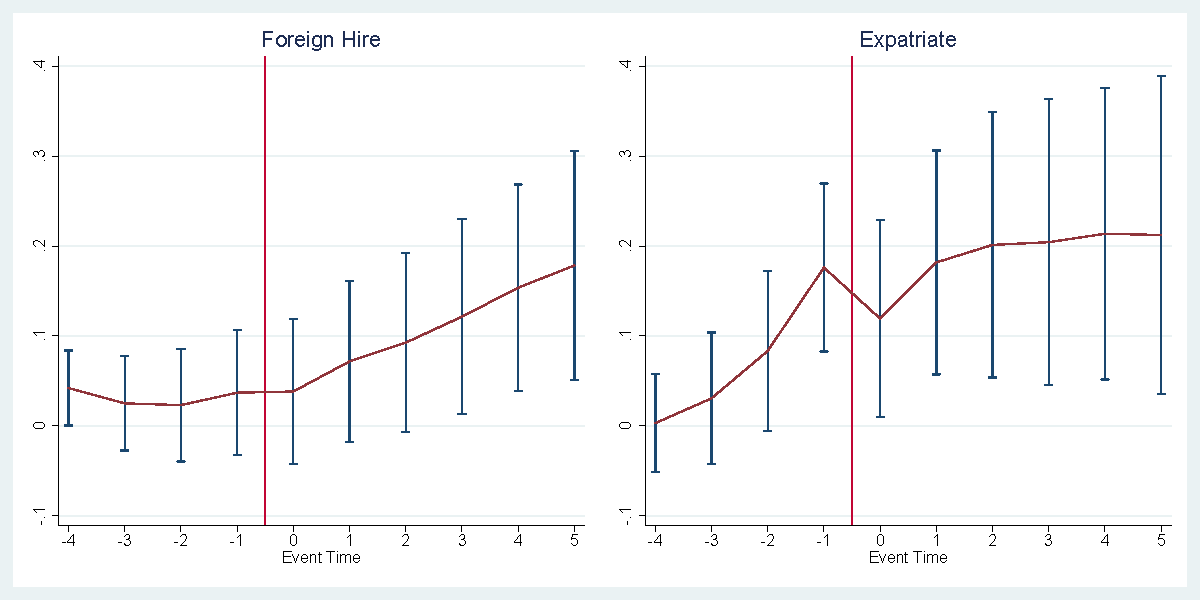
\includegraphics[width=15cm]{Regression/gr_lnQ.pdf}
\caption*{The figure presents the estimated coefficients and confidence intervals associated with the 5-percent levels of significance of foreign hired local and expatriate mangers on the scale of production by event-time (year 0 = the year when the manager became CEO. Regression attributes as in the notes of Table \ref{table:direct_effect_1}.}
\end{figure}

\begin{figure}
\center
\caption{The Effect of Managers on Labor Productivity (Event Time Estimations)}
\label{figure:dynamics_lnQL}
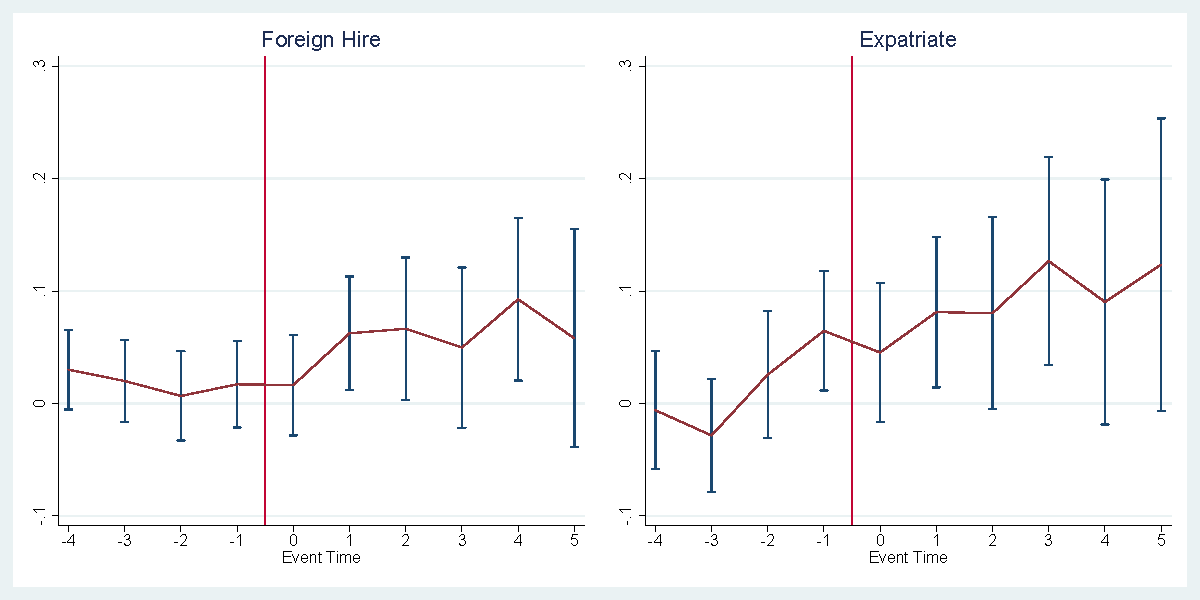
\includegraphics[width=15cm]{Regression/gr_lnQL.pdf}
\caption*{The figure presents the estimated coefficients and confidence intervals associated with the 5-percent levels of significance of foreign hired local and expatriate mangers on the scale of production by event-time (year 0 = the year when the manager became CEO. Regression attributes as in the notes of Table \ref{table:direct_effect_1}.}
\end{figure}

\begin{figure}
\caption{The Effect of Managers on TFP (Event Time Estimations)}
\label{figure:dynamics_exporter_5}
\center
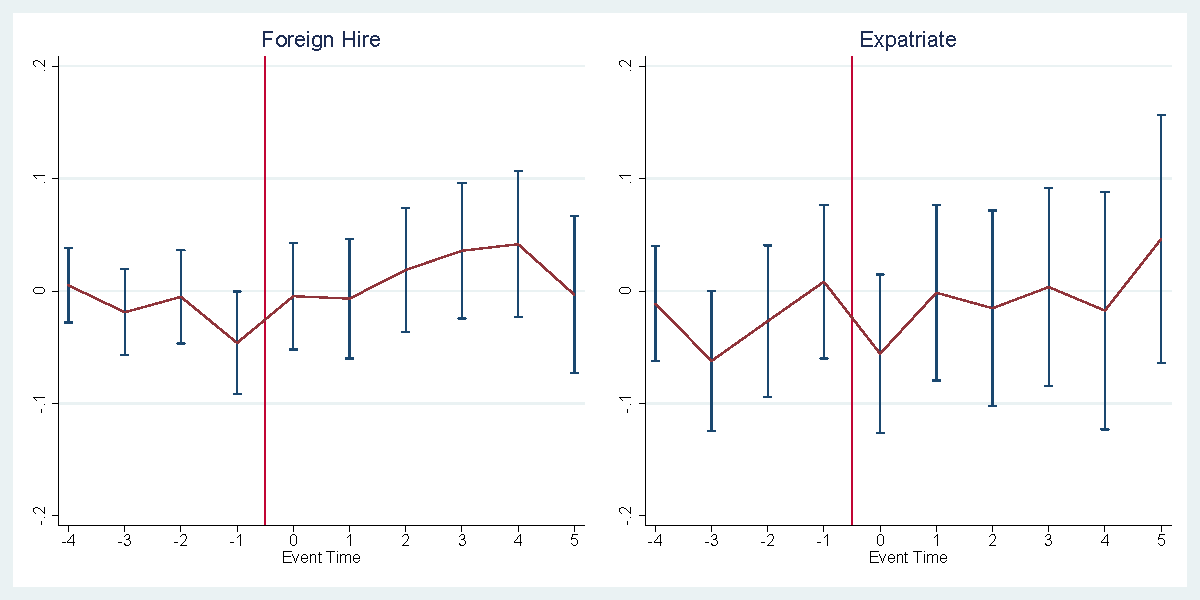
\includegraphics[width=15cm]{Regression/gr_TFP.pdf}
\caption*{The figure presents the estimated coefficients and confidence intervals associated with the 5-percent levels of significance of foreign hired local and expatriate mangers on the scale of production by event-time (year 0 = the year when the manager became CEO. Regression attributes as in the notes of Table \ref{table:direct_effect_1}.  }
\end{figure}

Is managerial performance effect linked to the CEO or it is long lasting? Can the CEO induce so profound changes in the company that its behavior changes for the long run? We test this in Table \ref{table:long_effect_1} where we augment the specification with dummy variables that take the value of 1 for the period of 5 years after the CEO leaves the company. Foreign hired local CEOs have long lasting effect on labor productivity as the estimated coefficient associated with the period after the manager left is positive, statistically significant and as large as 0.124 (somewhat larger than the direct effect). Expatriate CEOs have long lasting effects on both the scale of production and productivity, and the magnitude of the coefficients are also larger for the period after the separation: sales increase continually by 10 percent annually after the CEO is replaced, while labor productivity raises by 8 percent. Exporting activity is different from the two other variables as the effect fades away as the expatriate CEO leaves the firm.

\begin{table}[h!]
\centering
\caption{Long Run Effects of Managers on Firm Performance}
\bigskip
\label{table:long_effect_1}
\begin{threeparttable}
{
\def\sym#1{\ifmmode^{#1}\else\(^{#1}\)\fi}
\begin{tabular}{l*{3}{D{.}{.}{-1}}}
\hline\hline
                    &\multicolumn{1}{c}{(1)}&\multicolumn{1}{c}{(2)}&\multicolumn{1}{c}{(3)}\\
                    &\multicolumn{1}{c}{Output}&\multicolumn{1}{c}{Labor Prod.}&\multicolumn{1}{c}{TFP}\\
\hline
Foreign Owned       &       0.141\sym{***}&       0.083\sym{***}&       0.033         \\
                    &     (0.031)         &     (0.020)         &     (0.032)         \\
[1em]
Foreign Hired CEO   &       0.020         &       0.056\sym{***}&       0.035         \\
                    &     (0.031)         &     (0.021)         &     (0.025)         \\
[1em]
Foreign Hired CEO Post&       0.062         &       0.091\sym{**} &       0.052         \\
                    &     (0.055)         &     (0.035)         &     (0.062)         \\
[1em]
Expatriate          &       0.124\sym{**} &       0.080\sym{***}&      -0.029         \\
                    &     (0.049)         &     (0.030)         &     (0.037)         \\
[1em]
Expatriate Post     &       0.237\sym{***}&       0.138\sym{***}&      -0.039         \\
                    &     (0.069)         &     (0.042)         &     (0.084)         \\
\hline
Observations        &      481360         &      481360         &       46617         \\
\(R^{2}\)           &       0.824         &       0.868         &       0.522         \\
\hline\hline
\end{tabular}
}

\begin{tablenotes}
			\small
      \item Notes: The unit of observation in the regression is a CEO-year. Time span for each CEO: 5 years before the start of service as CEO to 5 years after resigning. Number of firms: 19,497; number of firm-years = 209,664. The regression is weighted with the inverse of the number of CEOs in a firm-year. The regressions control for a set of firm age dummies, industry-year interactions and firm fixed-effects. Mean(exporting) = 0.22. Standard errors clustered at the firm level in parentheses. *** = significant at the 1-percent level; ** = significant at the 5-percent level; * = significant at the 10-percent level.}
    \end{tablenotes}
\end{threeparttable}
\end{table}

One long lasting effect of foreign hired domestic CEOs is that increases the likelihood of becoming exporter, while the direct effect of local CEOs is zero. One possible solution to this apparent contradiction is that local and expatriate CEOs sometimes replace each other and so the long term exporting effect of local CEOs coincides with the direct effect of the next (expatriate) manager. We test this in the next table when we directly estimate the effect on firm performance of CEOs when they switch between local and expatriate. We replace the foreign hire and expatriate variables with 4 other variables representing the type of switch between local and expatriate managers: local-local, local-expatriate, expatriate-local and expatriate-expatriate.\footnote{The variables refer to the identity of the new CEO. For example the local-expatriate variable equals 1 when the CEO is expatriate, while the preceding CEO was local.} 

Table \ref{table:switch_effect_1} shows the estimated coefficients associated with the switch type. Local CEOs raise productivity regardless of the identity of the previous CEO, but their effect is more than twice as large when they replace an expatriate (13.5 percent). In this case we find a scale effect of the local CEO of the magnitude of 8 percent which does not exist in the case of domestic-domestic switch. Turning to expatriates, we find positive effects which are significantly different from zero on all the three measures of performance regardless the previous CEOs identity, but they are much larger in magnitude when the switch is between to expatriate CEOs. For the scale of production, the effect 7.6 percent when locals are the preceding CEOs and 23.3 percent when expatriates; for productivity and exporting status the effect are twice as large when expatriates replace expatriates. It seems thus that while the foreign owners are better at selecting their CEOs in general, expatriates have long lasting effects which prevail in the period subsequent to the expatrate presence in the firm and this effect does not depend on the identity of the next CEO. 

\begin{table}[h!]
\centering
\caption{Effects of Managers Switching Between Locals and Expatriates}
\bigskip
\label{table:switch_effect_1}
\begin{threeparttable}
{
\def\sym#1{\ifmmode^{#1}\else\(^{#1}\)\fi}
\begin{tabular}{l*{3}{D{.}{.}{-1}}}
\hline\hline
                    &\multicolumn{1}{c}{(1)}&\multicolumn{1}{c}{(2)}&\multicolumn{1}{c}{(3)}\\
                    &\multicolumn{1}{c}{Output}&\multicolumn{1}{c}{Labor Prod.}&\multicolumn{1}{c}{TFP}\\
\hline
Foreign Owned       &       0.113\sym{***}&       0.061\sym{***}&      -0.010         \\
                    &     (0.023)         &     (0.016)         &     (0.015)         \\
[1em]
during\_foreign\_DD   &      -0.033         &       0.060\sym{**} &       0.018         \\
                    &     (0.036)         &     (0.024)         &     (0.018)         \\
[1em]
during\_foreign\_ED   &       0.208\sym{***}&       0.160\sym{***}&       0.060\sym{**} \\
                    &     (0.052)         &     (0.033)         &     (0.029)         \\
[1em]
during\_foreign\_DE   &       0.078         &       0.168\sym{***}&       0.024         \\
                    &     (0.056)         &     (0.034)         &     (0.034)         \\
[1em]
during\_foreign\_EE   &       0.170\sym{***}&       0.172\sym{***}&       0.035         \\
                    &     (0.049)         &     (0.033)         &     (0.029)         \\
\hline
Observations        &      408166         &      408166         &      362051         \\
\(R^{2}\)           &       0.837         &       0.879         &       0.546         \\
\hline\hline
\end{tabular}
}

\begin{tablenotes}
			\small
      \item Notes: The unit of observation in the regression is a CEO-year. Time span for each CEO: 5 years before the start of service as CEO to 5 years after resigning. Number of firms: 19,497; number of firm-years = 209,664. The regression is weighted with the inverse of the number of CEOs in a firm-year. The regressions control for a set of firm age dummies, industry-year interactions and firm fixed-effects. Mean(exporting) = 0.22. Standard errors clustered at the firm level in parentheses. *** = significant at the 1-percent level; ** = significant at the 5-percent level; * = significant at the 10-percent level.}
    \end{tablenotes}
\end{threeparttable}
\end{table}

\subsection{Changes within the Firm: Capital, Intermediate Inputs, Structure of Employment and Wages}
Having established the performance effects of CEOs appointed by foreign owners, we now try to understand what induces the increase in sales, labor productivity and exporting activity. For this we study the utilization of inputs that are usually included in standard production functions, such as capital, labor and material costs. Next, employ our employee-level data to take a closer look at the utilization of labor. We first disentangle labor into three types (skilled, medium skilled and unskilled) and we also analyze the wages of the three groups. Relative wages may shed light on the relative marginal productivity of the three groups and its change as the new CEO changes the organization of the firm.

First we look at the utilization of capital. One potential advantage of foreign ownership pointed out by policy makers and researchers as well at the beginning of the transition from the command economy to a capitalist system was the hope that the parent companies would inject the old socialist enterprises with new capital and advanced technologies (ref). To test whether this is true, we run the same regressions as before but with the log value of tangible assets and log capital-labor ratio as dependent variables. Such changes would hint towards an upgrading of technology and switch to more capital intensive modes of production (such as the robotization of production process). As the first two column of Table \ref{table:direct_effect_2} demonstrates, we fail to find such mechanisms. Only local CEOs hired after the acquisitions employ more capital than similar domestic companies, and the difference is economically small (1 percentage point or 14 percent, evaluated at the mean investment). Nor the level of employment is affected by the newly elected CEOs. As a consequence of the stability of the levels of capital and labor, the capital-labor ratio is also stable. It seems thus that the levels of the two most important factors of production -- capital and labor -- do not play an important role in the process of improvement of the value of sales and firm productivity.

The last column of Table \ref{table:direct_effect_2} presents the last major input for the firm, the costs of intermediate inputs. Similar to the capital-labor ratio and labor productivity, we scale this variable with the number of employees in the firm. Unlike the other two factors, both foreign ownership and management has large effects on this ratio. Foreign acquisitions that are not accompanied with changes in the CEO have an associated effect of 9.2 percent. This effect increases by 7 percent when new local CEOs lead the company and an additional 8.5 percent when the new CEO is an expat. Taken together, a company that is led by an expat manager increases its material expenditures per employee by 25 percent. According to these estimations, the first reason for the higher output and labor productivity of foreign-owned companies is not capital or labor, but the quality of intermediate goods employed by the new owners. This effect is intensified if the foreign owners replace the CEO of the company and it further increases when the CEO is of foreign origin.

\begin{table}[h!]
\centering
\caption{The Effect of Managers on Input Utilization}
\bigskip
\label{table:direct_effect_2}
\begin{threeparttable}
{
\def\sym#1{\ifmmode^{#1}\else\(^{#1}\)\fi}
\begin{tabular}{l*{4}{D{.}{.}{-1}}}
\hline\hline
            &\multicolumn{1}{c}{(1)}&\multicolumn{1}{c}{(2)}&\multicolumn{1}{c}{(3)}&\multicolumn{1}{c}{(4)}\\
            &\multicolumn{1}{c}{invest\_10}&\multicolumn{1}{c}{lnL}&\multicolumn{1}{c}{lnKL}&\multicolumn{1}{c}{lnML}\\
\hline
foreign     &       0.002         &       0.012         &       0.103\sym{***}&       0.092\sym{***}\\
            &     (0.004)         &     (0.027)         &     (0.032)         &     (0.021)         \\
[1em]
during      &      -0.000         &       0.004         &       0.016\sym{**} &       0.000         \\
            &     (0.001)         &     (0.006)         &     (0.007)         &     (0.005)         \\
[1em]
during\_foreign&       0.010\sym{***}&      -0.029         &      -0.112\sym{***}&       0.071\sym{***}\\
            &     (0.003)         &     (0.028)         &     (0.031)         &     (0.021)         \\
[1em]
during\_expat&       0.002         &       0.021         &       0.029         &       0.085\sym{***}\\
            &     (0.004)         &     (0.038)         &     (0.041)         &     (0.030)         \\
\hline
\(N\)       &      464090         &      482421         &      464090         &      461186         \\
\(R^{2}\)   &       0.155         &       0.691         &       0.763         &       0.849         \\
\hline\hline
\end{tabular}
}

\begin{tablenotes}
			\small
      \item Notes: The unit of observation in the regression is a CEO-year. Time span for each CEO: 5 years before the start of service as CEO to 5 years after resigning. Number of firms: 19,497; number of firm-years = 209,664. The regression is weighted with the inverse of the number of CEOs in a firm-year. The regressions control for a set of firm age dummies, industry-year interactions and firm fixed-effects. Mean(exporting) = 0.22. Standard errors clustered at the firm level in parentheses. *** = significant at the 1-percent level; ** = significant at the 5-percent level; * = significant at the 10-percent level.}
    \end{tablenotes}
\end{threeparttable}
\end{table}

Another channel of productivity improvement is not the level, but quality of, emplyoment. It is possible, for example, that the new managers do not change the number of employees but they alter the proportion of high-skilled workers. As Table \ref{table:employment_effect} shows, this is not the case in our data. We run our baseline specification on the employee sample with three dummy variables as dependent variables showing whether the employee has at least collage degree, is graduated from a high school or has less than high school level of completed education. 


\begin{table}[h!]
\centering
\caption{Effects of Managers on Employment Outcomes}
\bigskip
\label{table:employment_effect}
\begin{threeparttable}
{
\def\sym#1{\ifmmode^{#1}\else\(^{#1}\)\fi}
\begin{tabular}{l*{6}{D{.}{.}{-1}}}
\hline\hline
                    &\multicolumn{1}{c}{(1)}&\multicolumn{1}{c}{(2)}&\multicolumn{1}{c}{(3)}&\multicolumn{1}{c}{(4)}&\multicolumn{1}{c}{(5)}&\multicolumn{1}{c}{(6)}\\
                    &\multicolumn{1}{c}{univ}&\multicolumn{1}{c}{high}&\multicolumn{1}{c}{low}&\multicolumn{1}{c}{lnW}&\multicolumn{1}{c}{lnW}&\multicolumn{1}{c}{lnW}\\
\hline
Foreign             &       0.007\sym{*}  &      -0.007         &      -0.000         &       0.056\sym{**} &       0.029\sym{**} &       0.032\sym{***}\\
                    &     (0.004)         &     (0.006)         &     (0.006)         &     (0.023)         &     (0.012)         &     (0.009)         \\
[1em]
during\_foreign      &       0.008\sym{**} &       0.000         &      -0.008         &       0.023         &       0.010         &       0.019\sym{*}  \\
                    &     (0.004)         &     (0.006)         &     (0.006)         &     (0.018)         &     (0.012)         &     (0.011)         \\
[1em]
during\_expat        &       0.003         &      -0.012         &       0.009         &      -0.019         &       0.017         &      -0.009         \\
                    &     (0.006)         &     (0.008)         &     (0.008)         &     (0.023)         &     (0.012)         &     (0.013)         \\
\hline
Observations        &     1671987         &     1671987         &     1672172         &      198180         &      524243         &      943707         \\
\(R^{2}\)           &       0.154         &       0.137         &       0.205         &       0.865         &       0.893         &       0.928         \\
\hline\hline
\end{tabular}
}

\begin{tablenotes}
			\small
      \item Notes: The unit of observation in the regression is a CEO-year. Time span for each CEO: 5 years before the start of service as CEO to 5 years after resigning. Number of firms: 19,497; number of firm-years = 209,664. The regression is weighted with the inverse of the number of CEOs in a firm-year. The regressions control for a set of firm age dummies, industry-year interactions and firm fixed-effects. Mean(exporting) = 0.22. Standard errors clustered at the firm level in parentheses. *** = significant at the 1-percent level; ** = significant at the 5-percent level; * = significant at the 10-percent level.}
    \end{tablenotes}
\end{threeparttable}
\end{table}

\section{Conclusion}
Using exhaustive administrative data from Hungary 1992--2014, we study the performance of firms led by expatriate managers. Studying more than 2,000 foreign acquisitions and more than 3,000 greenfield foreign investments, we compare firms that bring in foreign management to those that remain locally managed. Foreign managed firms improve their productivity faster. Larger, more capital intensive and more productive firms are more likely to receive a foreign manager. Owners from distant countries and tax havens are more likely to leave domestic management in place. 

Given the potential benefits of good management, it is puzzling that many firms do not upgrade their management practices, even given low-cost opportunities to do so \cite{Bloom2012-ek}. Are management needs specific to the firm? Evidence from CEOs moving across corporations reveals that managers differ in “style,” and they adopt different management practices \cite{Bertrand2003-io,Schoar2016-rj}. There is also evidence that managers moving across firms transfer specific knowledge. \cite{Mion2014-vi} show that managers leaving exporting firms increase the propensity of exports in their new host company. In previous work \cite{Bisztray2016-iq}, we documented similar patterns for importing firms, even after controlling for spatial and ownership links.

Our work suggests that \emph{managers}, not only \emph{management} matters and can provide a link between foreign ownership and management practices.

\bibliography{references_2}

\end{document} 